\section{Introduction}
Parallel and distributed computing are a staple of modern applications. We need to leverage multiple cores or multiple machines to speed up applications or to run them at a large scale. The infrastructure for crawling the web and responding to search queries are not single-threaded programs running on someone’s laptop but rather collections of services that communicate and interact with one another.

The cloud promises unlimited scalability in all directions (memory, compute, storage, etc). Realizing this promise requires new tools for programming the cloud and building distributed applications.

\begin{figure}[!htbp]
    \centering
    
\includegraphics[width=\textwidth]{ray-logo}
\end{figure}

To task advantage of this unlimited scalability this experiment aims towards building application with Ray Framework build in python which can scale from \verb|laptop to large cluster|.


\subsection{Significance of Ray}
Ray is capable to handle requirements of modern days application listed below:
\begin{itemize}
    \item Running the same code on more than one machine.
    \item Building micro-services and actors that have state and can communicate.
    \item Gracefully handling machine failures.
    \item Efficiently handling large objects and numerical data.
\end{itemize}

Traditional Programming rely on 2 core concepts:
\begin{itemize}
    \item functions
    \item classes
\end{itemize}
Using these building blocks, programming languages allow us to build countless applications.

However, when we migrate our applications to the distributed setting, the concepts typically change.

On one end of the spectrum, we have tools like \href{https://www.open-mpi.org/}{OpenMPI}, \verb|Python multiprocessing|, and \href{http://zeromq.org/}{ZeroMQ}, which provide low-level primitives for sending and receiving messages. These tools are very powerful, but they provide a different abstraction and so single-threaded applications must be rewritten from scratch to use them.

On the other end of the spectrum, we have domain-specific tools like \href{https://www.tensorflow.org/}{TensorFlow} for model training, \href{https://spark.apache.org/}{Spark} for data processing and SQL, and \href{https://flink.apache.org/}{Flink} for stream processing. These tools provide higher-level abstractions like neural networks, datasets, and streams. However, because they differ from the abstractions used for serial programming, applications again must be rewritten from scratch to leverage them.

\begin{figure}[!htbp]
    \centering
    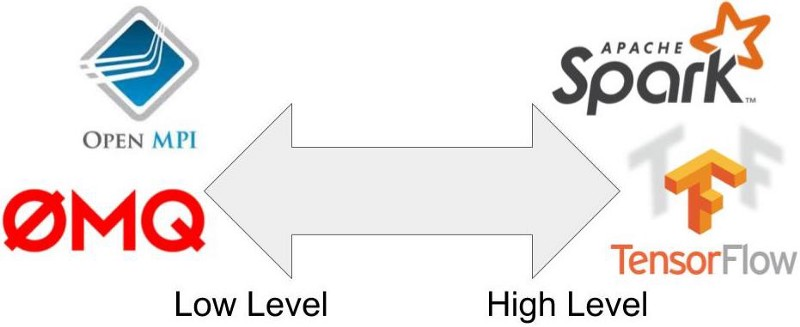
\includegraphics[width=0.7\textwidth]{distributed-computing-app}
    \caption{Tools for distributed computing on an axis from low-level primitives to high-level abstractions.}
\end{figure}

Ray occupies a unique middle ground. Instead of introducing new concepts. Ray takes the existing concepts of functions and classes and translates them to the distributed setting as tasks and actors. This API choice allows serial applications to be parallelized without major modifications.

\section{Introduction to Ray}
Ray is a distributed execution engine. The same code can be run on a single machine to achieve efficient multiprocessing, and it can be used on a cluster for large computations.

When using Ray, several processes are involved.

\begin{itemize}
    \item Multiple worker processes execute tasks and store results in object stores. Each worker is a separate process.
    \item One object store per node stores immutable objects in shared memory and allows workers to efficiently share objects on the same node with minimal copying and deserialization.
    \item One raylet per node assigns tasks to workers on the same node.
    \item A driver is the Python process that the user controls. For example, if the user is running a script or using a Python shell, then the driver is the Python process that runs the script or the shell. A driver is similar to a worker in that it can submit tasks to its raylet and get objects from the object store, but it is different in that the raylet will not assign tasks to the driver to be executed.
    \item A Redis server maintains much of the system’s state. For example, it keeps track of which objects live on which machines and of the task specifications (but not data). It can also be queried directly for debugging purposes.
\end{itemize}

\subsection{Initializing Ray}
To start Ray, start Python and run the following commands:
\begin{minted}{python}
import ray
ray.init()
\end{minted}

The \verb|ray.init()| command starts all of the relevant Ray processes. 

On a cluster, this is the only line that needs to change (we need to pass in the cluster address). These processes include the following:
\begin{itemize}
    \item A number of worker processes for executing Python functions in parallel (roughly one worker per CPU core).
    \item A scheduler process for assigning “tasks” to workers (and to other machines). A task is the unit of work scheduled by Ray and corresponds to one function invocation or method invocation.
    \item A shared-memory object store for sharing objects efficiently between workers (without creating copies).
    \item An in-memory database for storing metadata needed to rerun tasks in the event of machine failures.
\end{itemize}

Ray workers are separate processes as opposed to threads because support for multi-threading in Python is very limited due to the \href{https://wiki.python.org/moin/GlobalInterpreterLock}{global interpreter lock}.

\subsection{Asynchronous Computation in Ray}
Ray enables arbitrary Python functions to be executed asynchronously. This is done by designating a Python function as a remote function.

For example, a normal Python function looks like below:
\begin{minted}{python}
def add1(a, b):
    return a + b
\end{minted}

A remote function looks like this.
\begin{minted}{python}
@ray.remote
def add2(a, b):
    return a + b
\end{minted}

Whereas calling \verb|add1(1, 2)| returns \verb|3| and causes the Python interpreter to block until the computation has finished, calling \verb|add2.remote(1, 2)| immediately returns an object ID and creates a task. The task will be scheduled by the system and executed asynchronously (potentially on a different machine). When the task finishes executing, its return value will be stored in the object store.

The following simple example demonstrates how asynchronous tasks can be used to parallelize computation:

\begin{minted}{python}
import time

def foo():
    time.sleep(1)

@ray.remote
def bar():
    time.sleep(1)

# The following takes ten seconds.
[foo() for _ in range(10)]

# The following takes one second (assuming the system has at least ten CPUs).
ray.get([bar.remote() for _ in range(10)])
\end{minted}

There is a sharp distinction between submitting a task and executing the task. When a remote function is called, the task of executing that function is submitted to a raylet, and object IDs for the outputs of the task are immediately returned. However, the task will not be executed until the system actually schedules the task on a worker. Task execution is not done lazily. The system moves the input data to the task, and the task will execute as soon as its input dependencies are available and there are enough resources for the computation.

When a task is submitted, each argument may be passed in by value or by object ID. For example, these lines have the same behavior.

\begin{minted}{python}
add2.remote(1, 2)
add2.remote(1, ray.put(2))
add2.remote(ray.put(1), ray.put(2))
\end{minted}
